%!TEX TS-program = pdflatexmk

% Copyright (c) 2018 - 2022, Martin Scheidt (ISC license)
% Permission to use, copy, modify, and/or distribute this file for any purpose with or without fee is hereby granted, provided that the above copyright notice and this permission notice appear in all copies.

\documentclass[border=2]{standalone}

\usepackage[dev]{tikz-trackschematic}

\begin{document}
  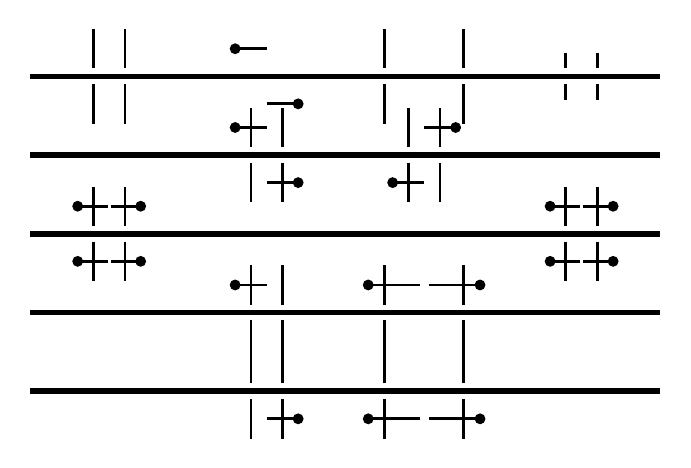
\begin{tikzpicture}
  
    \foreach \i in {1,2,...,5}{% base coordinate
      \coordinate (A\i) at ($(0,0) + (0,-\i)$);% base coordinate
      \coordinate (B\i) at ($(8,0) + (0,-\i)$);% base coordinate
    }

    \foreach \i in {1,2,...,5}{% draw main tracks on base coordinate
      \maintrack (A\i) --   (B\i);
    }

    \foreach \i in {1,2,...,5}{% coordinates for testing symbols
      \coordinate (X\i-1) at ($(1,0) + (0,-\i)$);
      \coordinate (X\i-2) at ($(3,0) + (0,-\i)$);
      \coordinate (X\i-3) at ($(5,0) + (0,-\i)$);
      \coordinate (X\i-4) at ($(7,0) + (0,-\i)$);
    }

    \levelcrossing[] at (X1-1);
    \levelcrossing[no road,barrier=semi] at (X1-2);
    \levelcrossing[road width=1cm] at (X1-3);
    \levelcrossing[width=0.2cm] at (X1-4);

    \levelcrossing[barrier=semi] at (X2-2);
    \levelcrossing[barrier=semi,position=left] at (X2-3);

    \levelcrossing[barrier=full] at (X3-1);
    \levelcrossing[barrier=full,position=left] at (X3-4);

    \levelcrossing[barrier=semi,side=left]  at (X4-2);
    \levelcrossing[barrier=semi,side=right] at (X5-2);

    \levelcrossing[road width=1cm,barrier=full,side=left]  at (X4-3);
    \levelcrossing[road width=1cm,barrier=full,side=right] at (X5-3);

  \end{tikzpicture}
\end{document}